\documentclass{article}

\usepackage{graphicx}
%\graphicspath{{./data/}}
\usepackage{float}

\title{Monte Carlo Integration Parallelization Report}
\author{Alejandro Servetto}

\begin{document}
\maketitle
\section{Methods}
I did the Monte Carlo techniqe.

I used the pthread library for my thread implementation. The way I parallelized
was to break up the summation. For \texttt{N} samples and \texttt{Nt} threads, I had each 
thread responsible for \texttt{N/Nt} samples of the summation. This was handled by a
subroutine \texttt{sum\_portion(float a, float b, int portion\_size, int n)}
where \texttt{portion\_size} is \texttt{N/Nt}. Each thread would enter its own little
subroutine, do its summation (with a thread safe random number generator) and write
its result to a heap-allocated array. Each thread was assigned an index of the array
to write to. The parent would wait for each baby thead to complete, look up the result
in the global array, and add it to the sum. When all threads completed and all of the
results were added to the sum, I normalized by multiplying \texttt{sum*(b-a)}.
Return result and print to stdout.

\section{Results}

I have access to a 40 core machine for my research, so I ran these on that. I picked arbitrary numbers
to do the integral on and for the sample size. Then did one run on each thread, recording the results.
You'll notice that there was a few times where a runtime was slightly faster than the previous...I'm
writing that off as sampling error, since it was only one trial each, and sometimes the OS prioritizes
a given process less frequently, given other external cicrumstances. This would probably
not be an issue if I and multiple iterations of each thread count and figured out the averages.

%\subsection{On 40 core machine}
\begin{figure}[H]
	\centering
	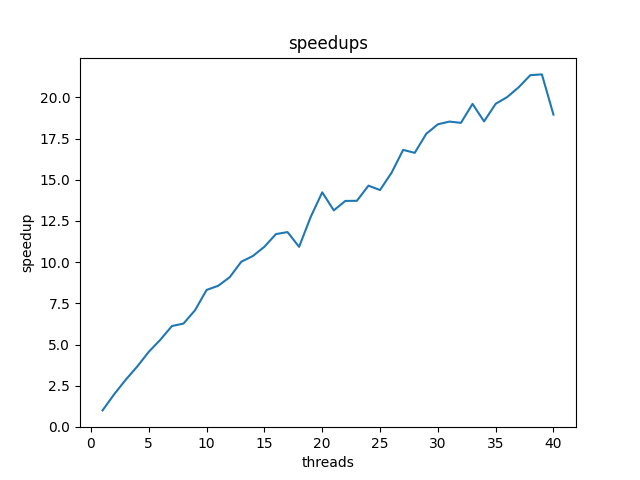
\includegraphics[width=10cm,height=10cm,keepaspectratio]{data/jolteon-plot-speedup.png}
	\caption{Speedup}
\end{figure}
\begin{figure}[H]
	\centering
	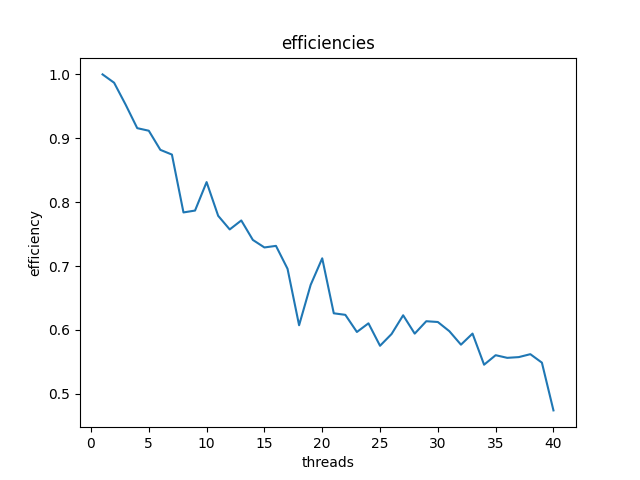
\includegraphics[width=10cm,height=10cm,keepaspectratio]{data/jolteon-plot-efficiency.png}
	\caption{Efficiency}
\end{figure}

%\subsection{On Remote.CS}
%\begin{figure}[H]
%	\centering
%	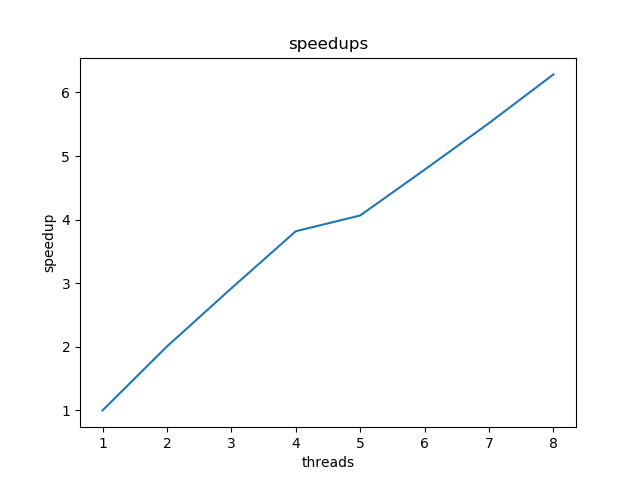
\includegraphics[width=10cm,height=10cm,keepaspectratio]{remotecs/tmp-speedup.png}
%	\caption{Speedup}
%\end{figure}
%\begin{figure}[H]
%	\centering
%	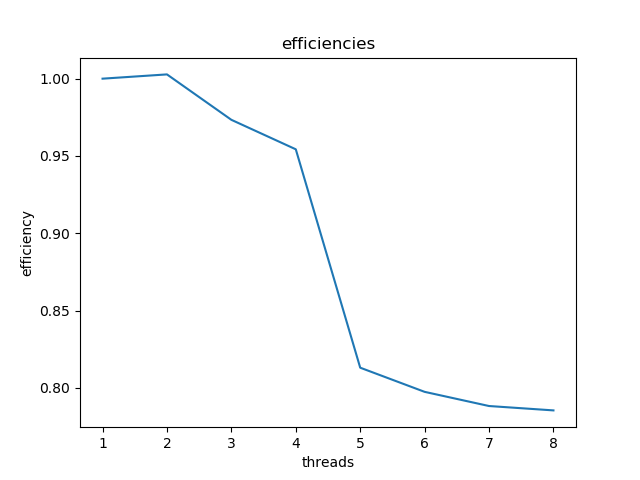
\includegraphics[width=10cm,height=10cm,keepaspectratio]{remotecs/tmp-efficiency.png}
%	\caption{Efficiency}
%\end{figure}

\section{Discussion}

%Looks like the addition of threads logarithmically increases runtime. It gets better,
%but by less and less. The only dramatic results were on the addition of the first
%few threads.

Looks like the speedup is linear, but not one-to-one. For example, at 20 threads, you only
get around a 15 times speedup. And it gets worse the more threads you add. This is also
demonstrated with the efficiency; it decreases with every added thread, although it stays
linear. So while each thread provided an additional speedup (minus error explained above,
likely because of exernal OS scheduling circumstances for a given process), each thread
was less helpful in making the computation faster.

\end{document}


